\section{Contribuições da UFFS}

% Trabalho da Gabrielle
\begin{frame}{Geração Procedural de Cânions Baseado em Ruído de Perlin}
  \begin{itemize}
        \item A partir de uma classificação de características de cânions;
        \item As características mais comuns foram selecionadas.
    \end{itemize}
\end{frame}

\begin{frame}{Geração Procedural de Cânions Baseado em Ruído de Perlin}
  \begin{figure}
		\centering
        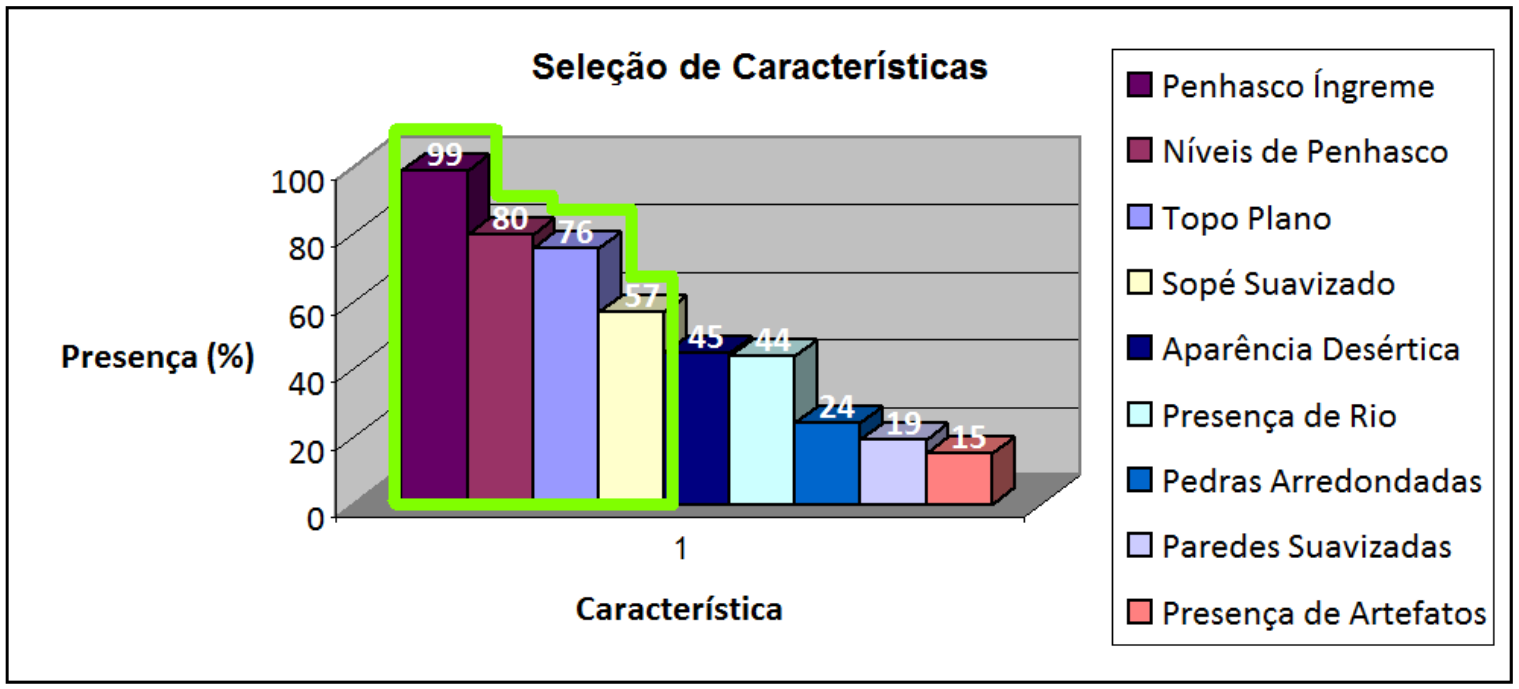
\includegraphics[width=.8\textwidth]{img/uffs/caract.png}
        \caption{Frequência de características nos cânions 
        \cite{gabrielle2016canion}.}
  \end{figure}
\end{frame}

\begin{frame}{Geração Procedural de Cânions Baseado em Ruído de Perlin}
  \begin{figure}
		\centering
        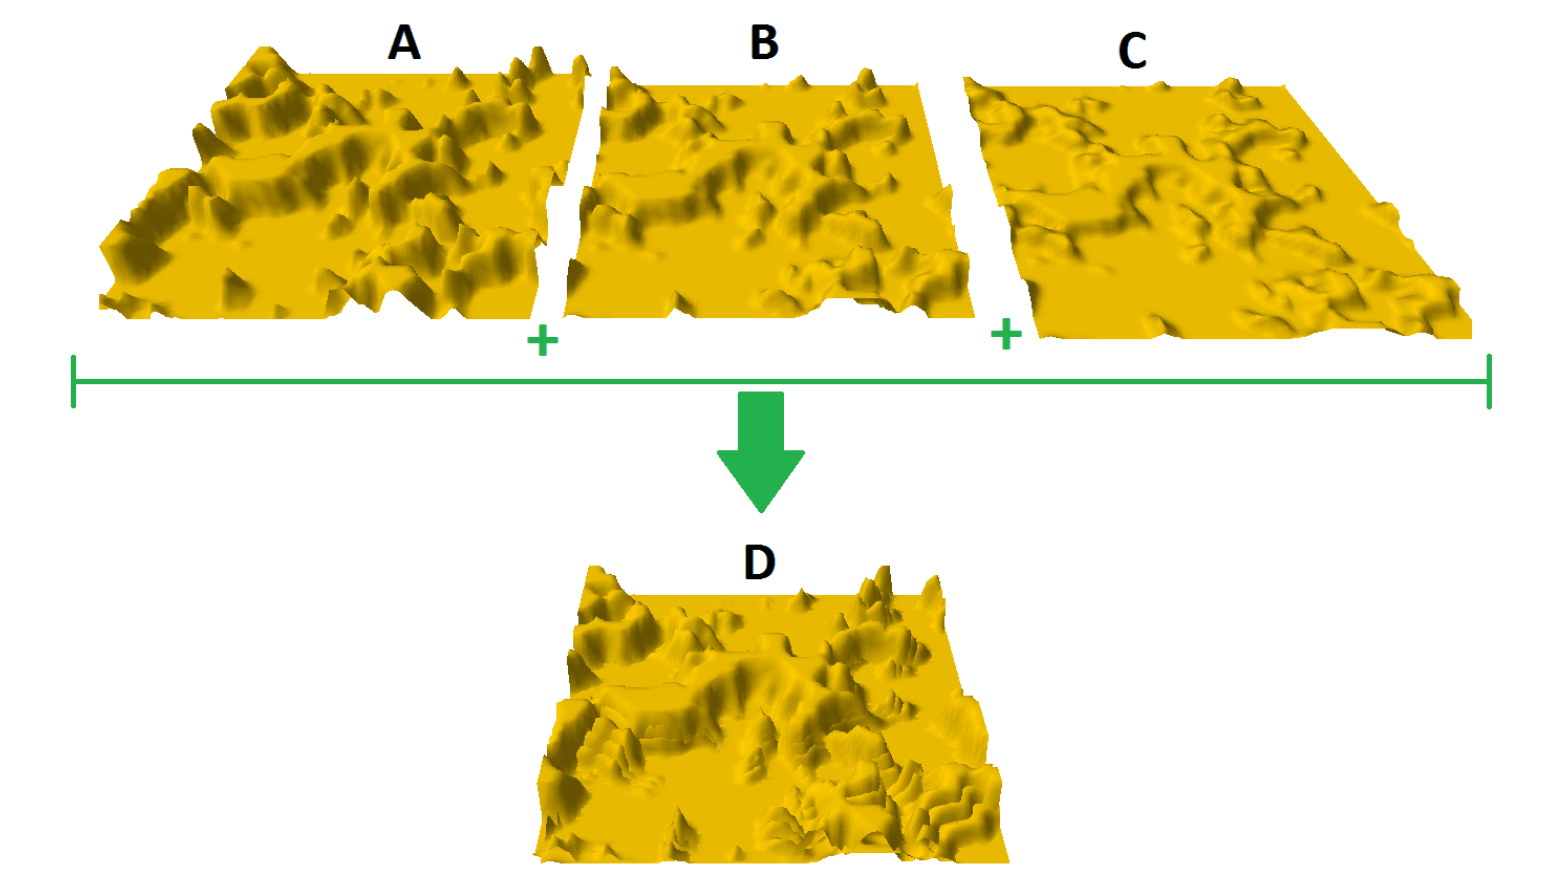
\includegraphics[width=.8\textwidth]{img/uffs/gabrielleDev.png}
        \caption{Soma das camadas para gerar Cânions}
  \end{figure}
\end{frame}

\begin{frame}{Geração Procedural de Cânions Baseado em Ruído de Perlin}
  \begin{figure}
		\centering
        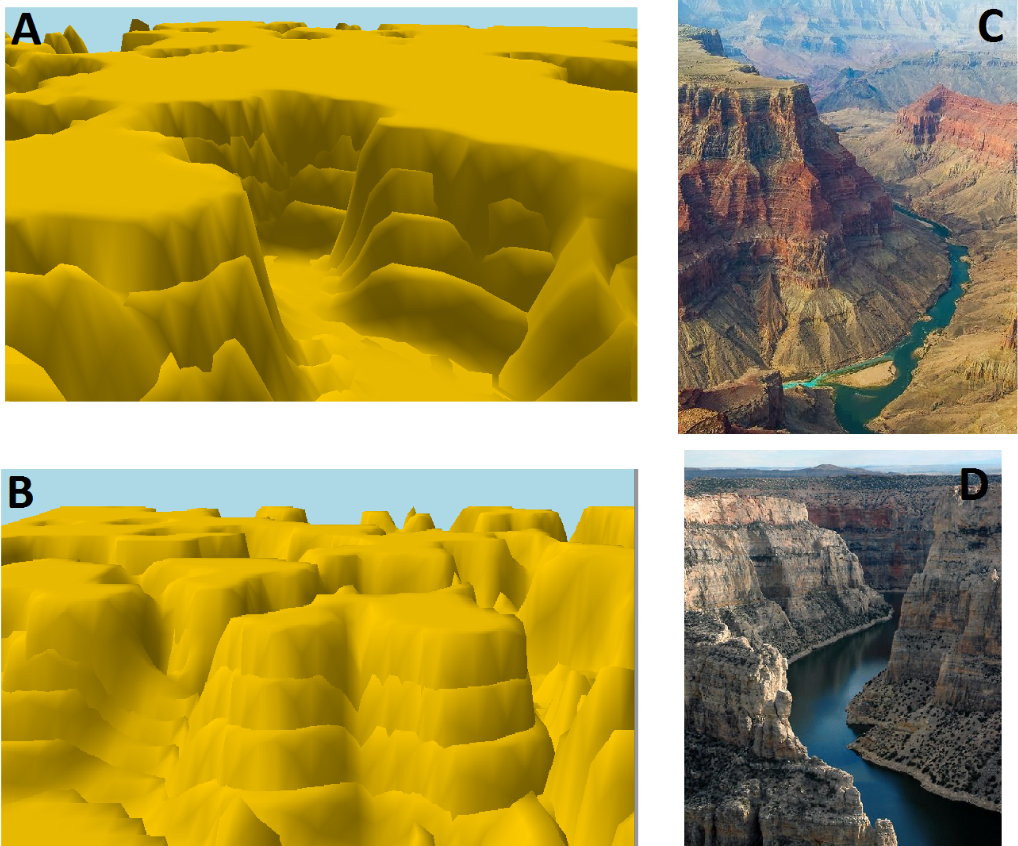
\includegraphics[width=.65\textwidth]{img/uffs/gabrielleResultado.png}
        \caption{Resultado Final}
  \end{figure}
\end{frame}


% Meu trabalho
\begin{frame}{Geração de Terrenos com Biomas Distintos para Jogos}
    \begin{itemize}
        \item Implementação de relevo para 5 \alert{Biomas}
            \begin{itemize}
                \item Planícies
                \item Montanhas
                \item Vales
                \item Deserto
                \item Cânyons
            \end{itemize}
        \item Distribuição dos Biomas
        \item Suavização das fronteiras
    \end{itemize}
\end{frame}

\begin{frame}{Geração de Terrenos com Biomas Distintos para Jogos}
  \begin{figure}
		\centering
        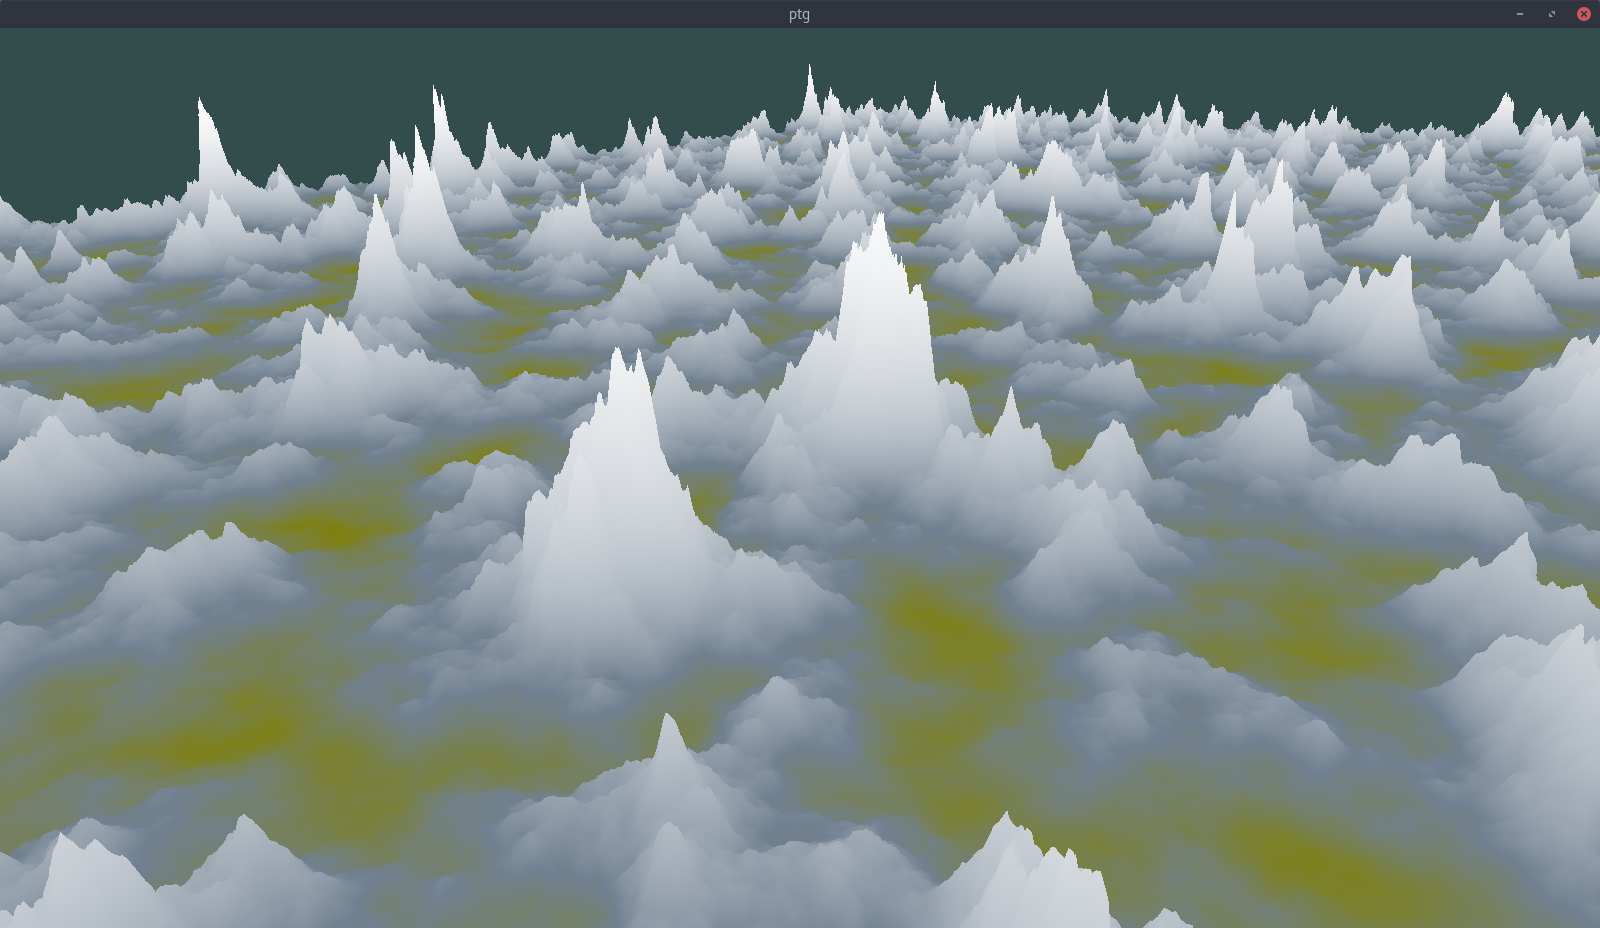
\includegraphics[width=.8\textwidth]{img/uffs/bssMontains.png}
        \caption{Montanhas}
  \end{figure}
\end{frame}

\begin{frame}{Geração de Terrenos com Biomas Distintos para Jogos}
  \begin{figure}
		\centering
        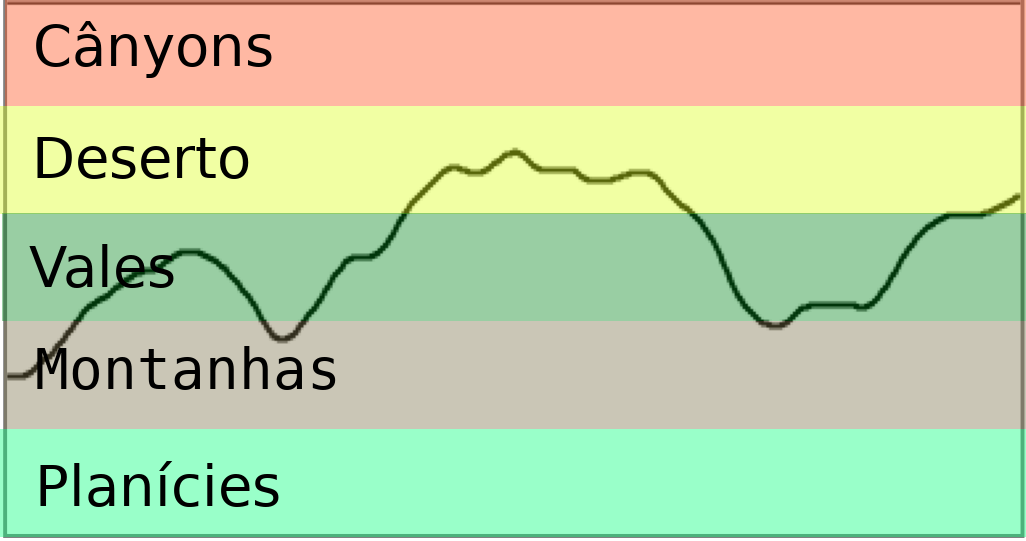
\includegraphics[width=.8\textwidth]{img/uffs/biomesdistnoise.png}
        \caption{Distribuição de Biomas}
  \end{figure}
\end{frame}

\begin{frame}{Geração de Terrenos com Biomas Distintos para Jogos}
  \begin{figure}
		\centering
        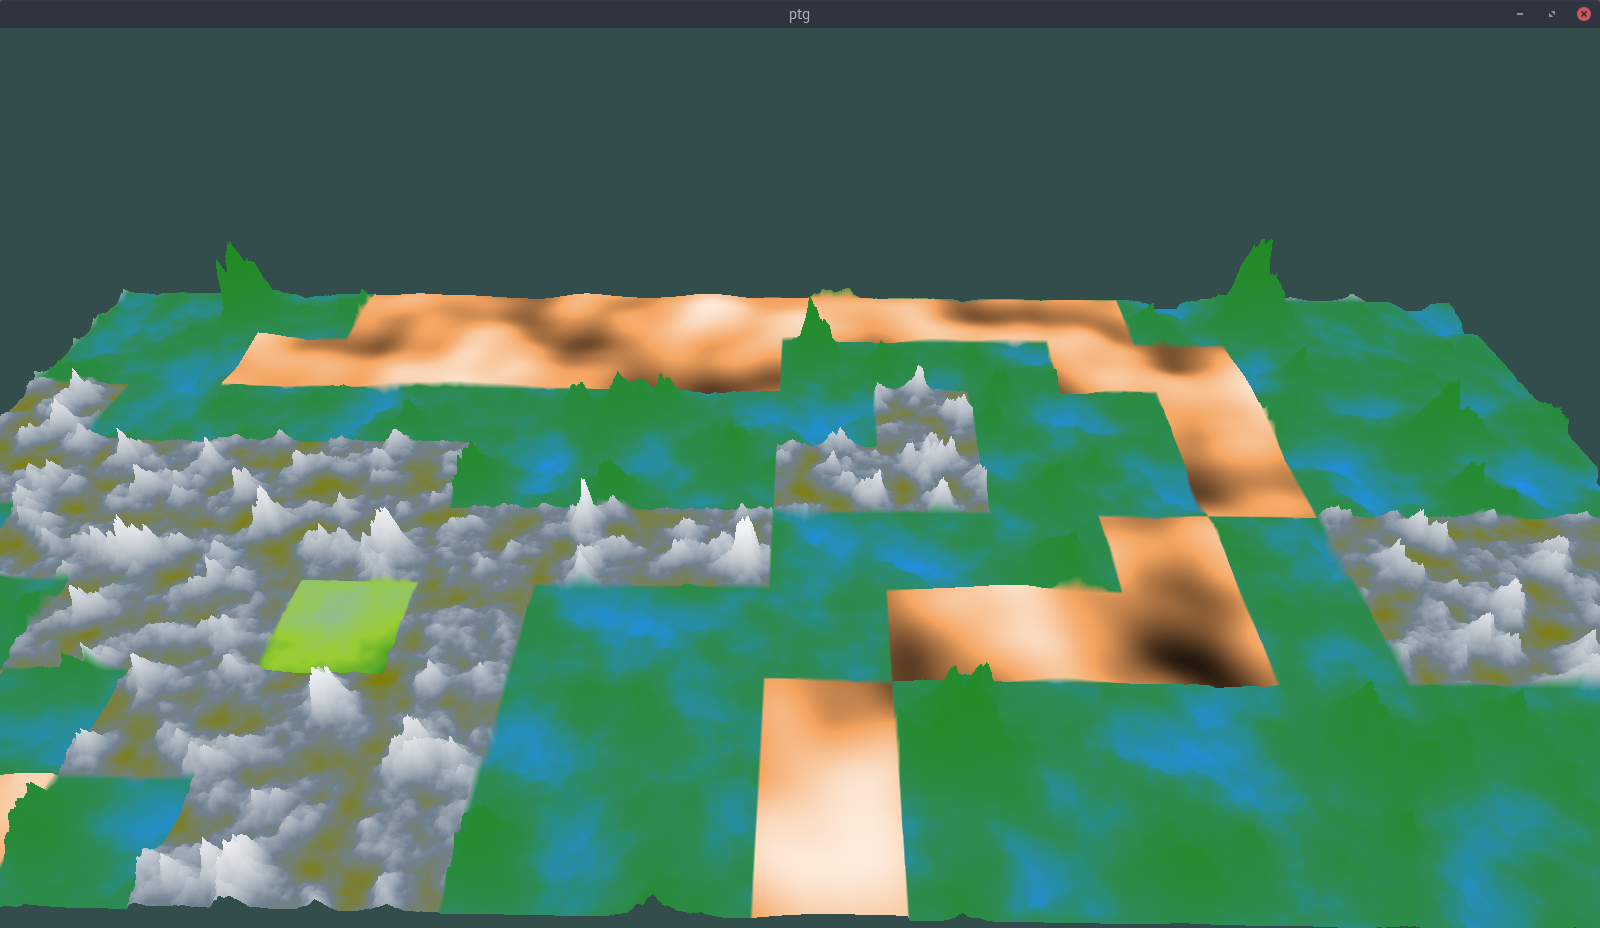
\includegraphics[width=.8\textwidth]{img/uffs/256f4.png}
        \caption{Distribuição de Biomas}
  \end{figure}
\end{frame}

\begin{frame}{Geração de Terrenos com Biomas Distintos para Jogos}
  \begin{figure}
		\centering
        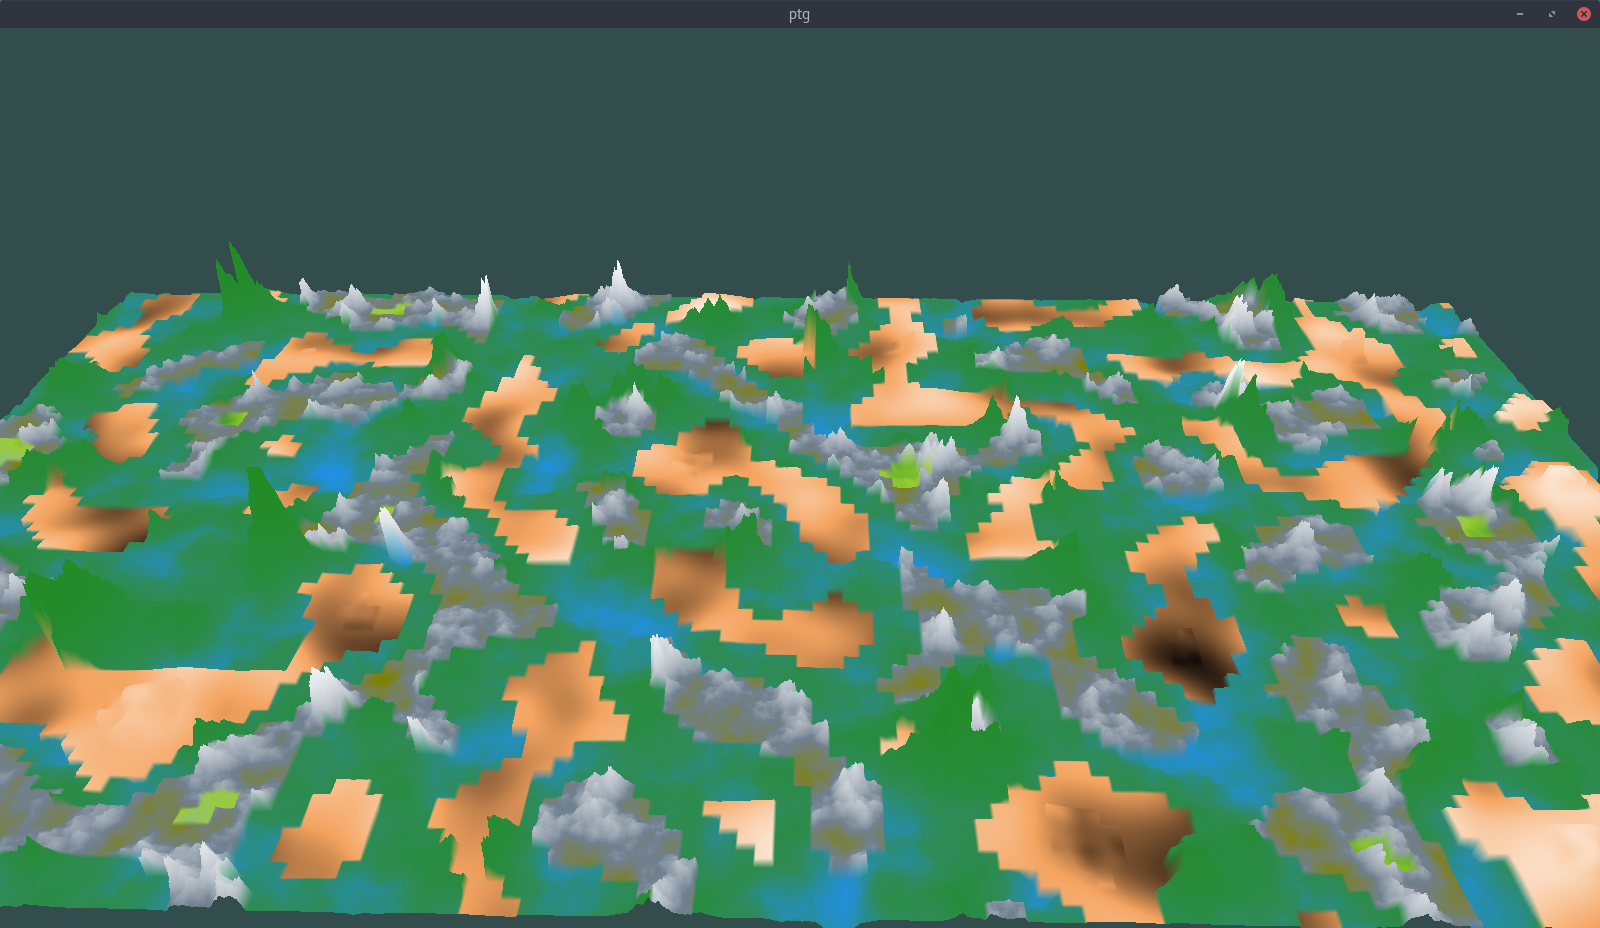
\includegraphics[width=.8\textwidth]{img/uffs/8b32.png}
        \caption{Frequência de Biomas = 8}
  \end{figure}
\end{frame}

\begin{frame}{Geração de Terrenos com Biomas Distintos para Jogos}
  \begin{figure}
		\centering
        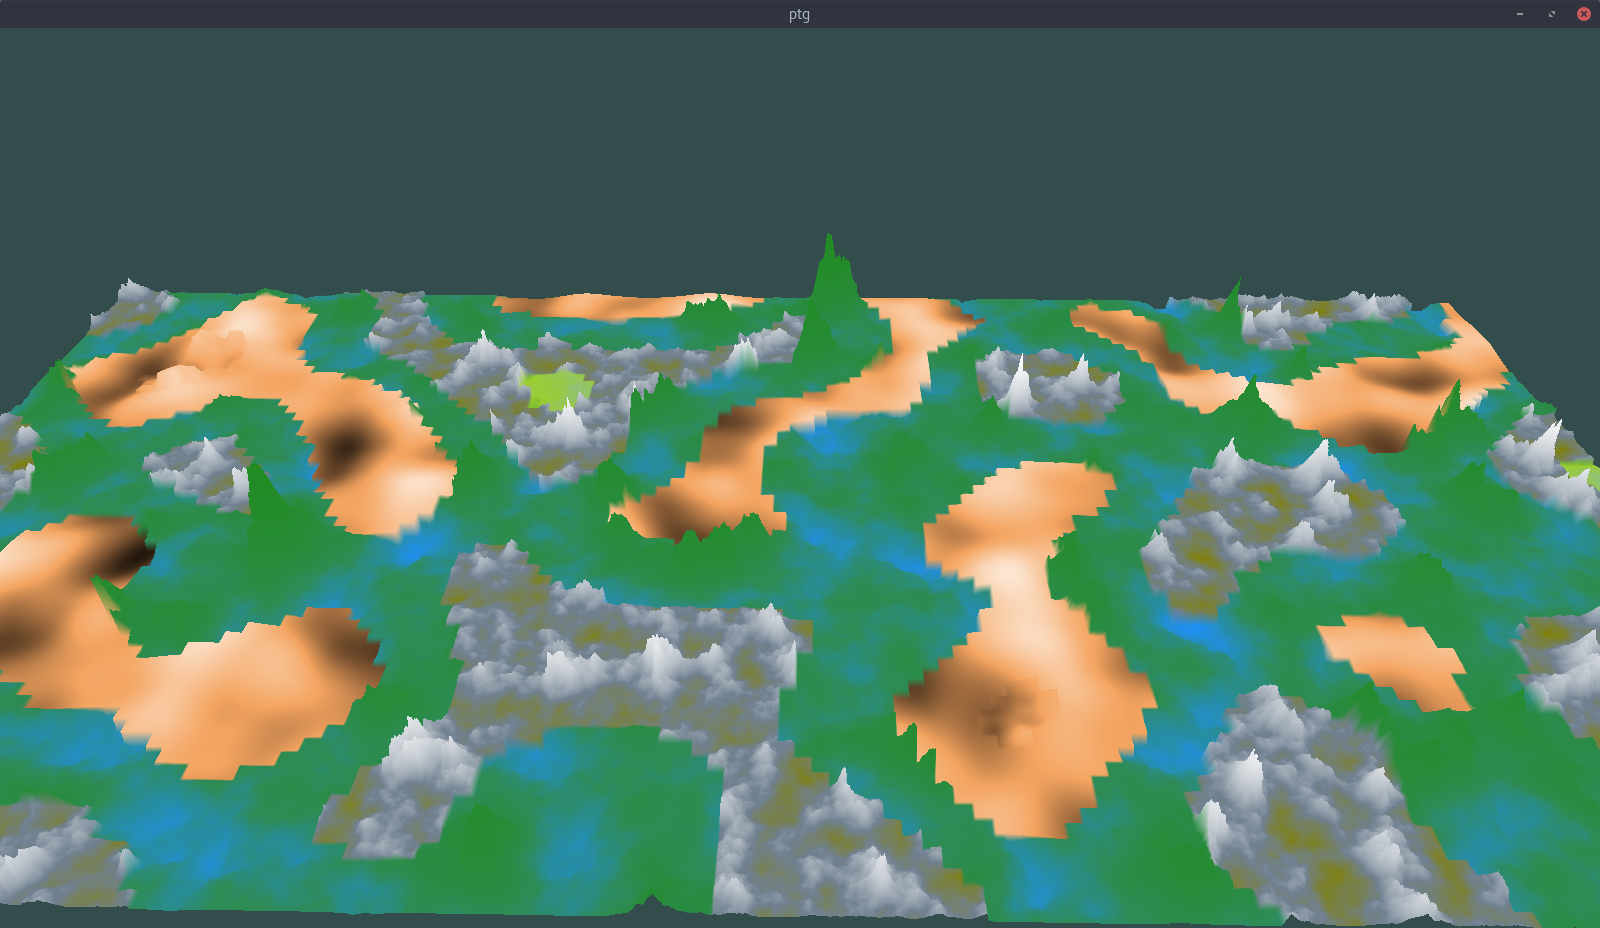
\includegraphics[width=.8\textwidth]{img/uffs/16b32.png}
        \caption{Frequência de Biomas = 16}
  \end{figure}
\end{frame}

\begin{frame}{Geração de Terrenos com Biomas Distintos para Jogos}
  \begin{figure}
		\centering
        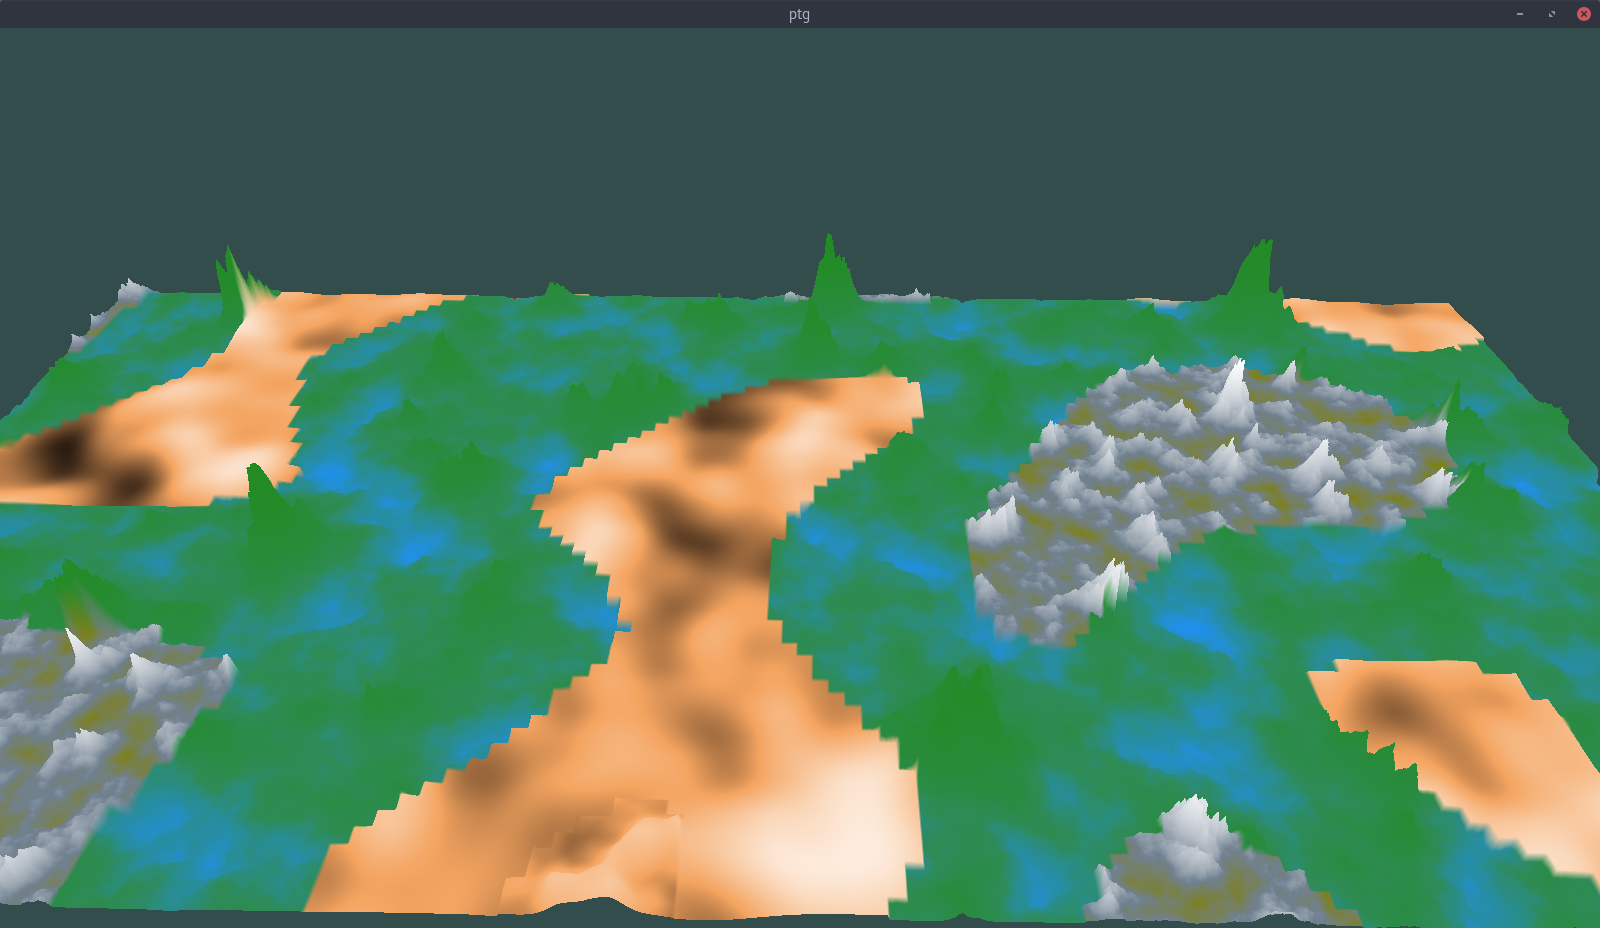
\includegraphics[width=.8\textwidth]{img/uffs/32b32.png}
        \caption{Frequência de Biomas = 32}
  \end{figure}
\end{frame}

\begin{frame}{Geração de Terrenos com Biomas Distintos para Jogos}
  \begin{figure}
		\centering
        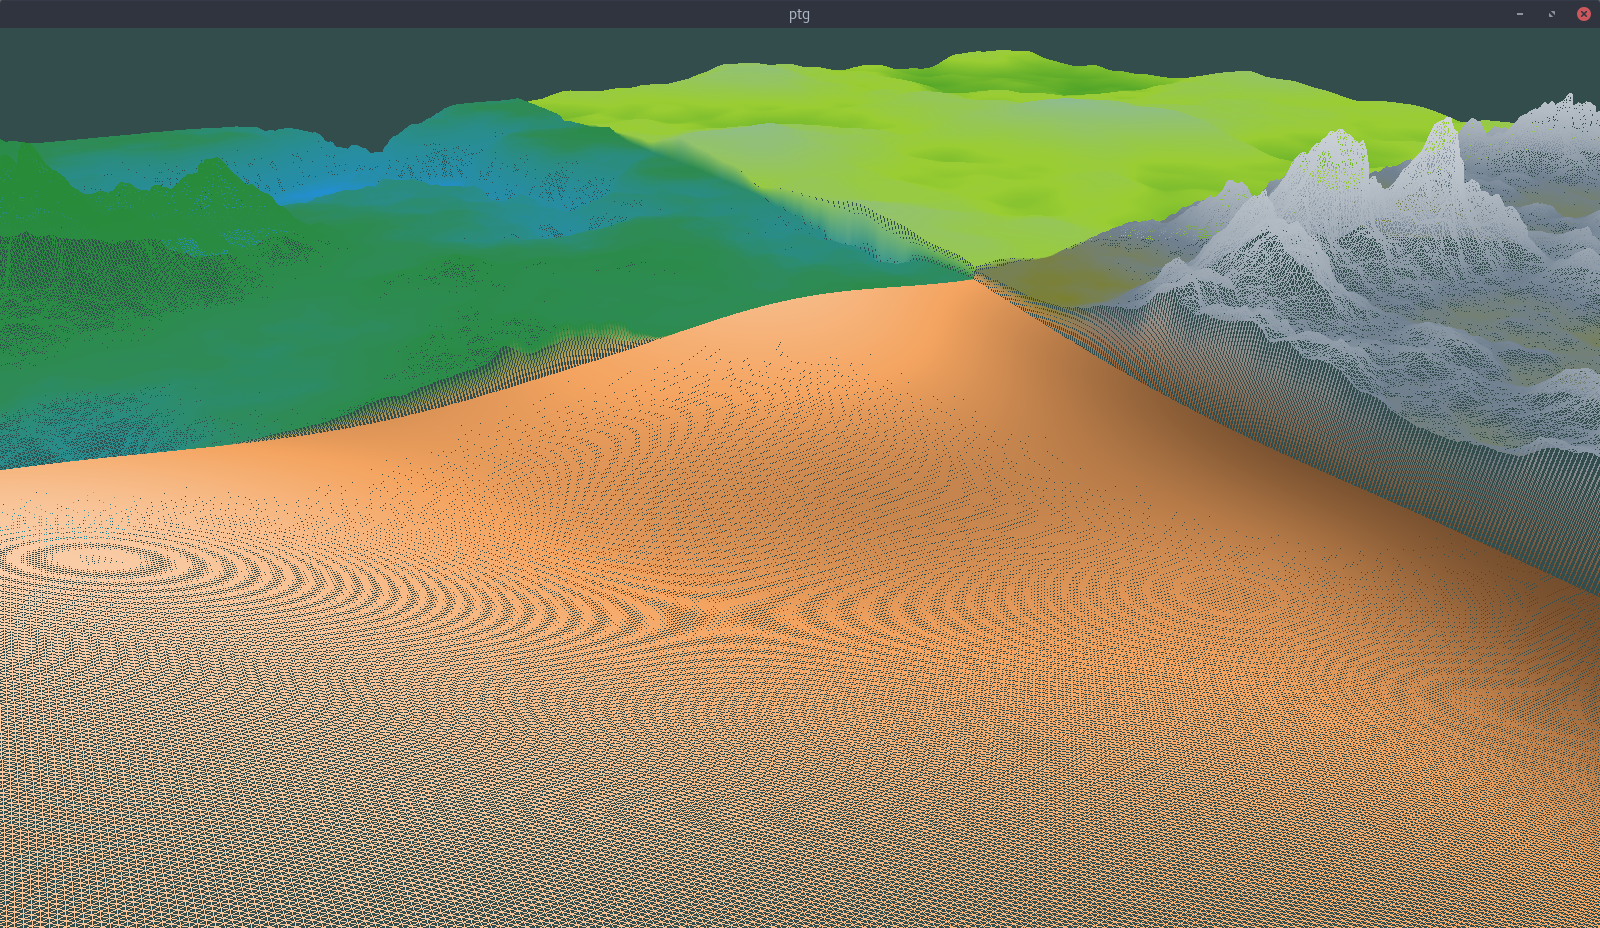
\includegraphics[width=.8\textwidth]
        {img/uffs/interpolationArea/notinter.png}
        \caption{Fronteiras descontínuas}
  \end{figure}
\end{frame}

\begin{frame}{Geração de Terrenos com Biomas Distintos para Jogos}
  \begin{figure}
		\centering
        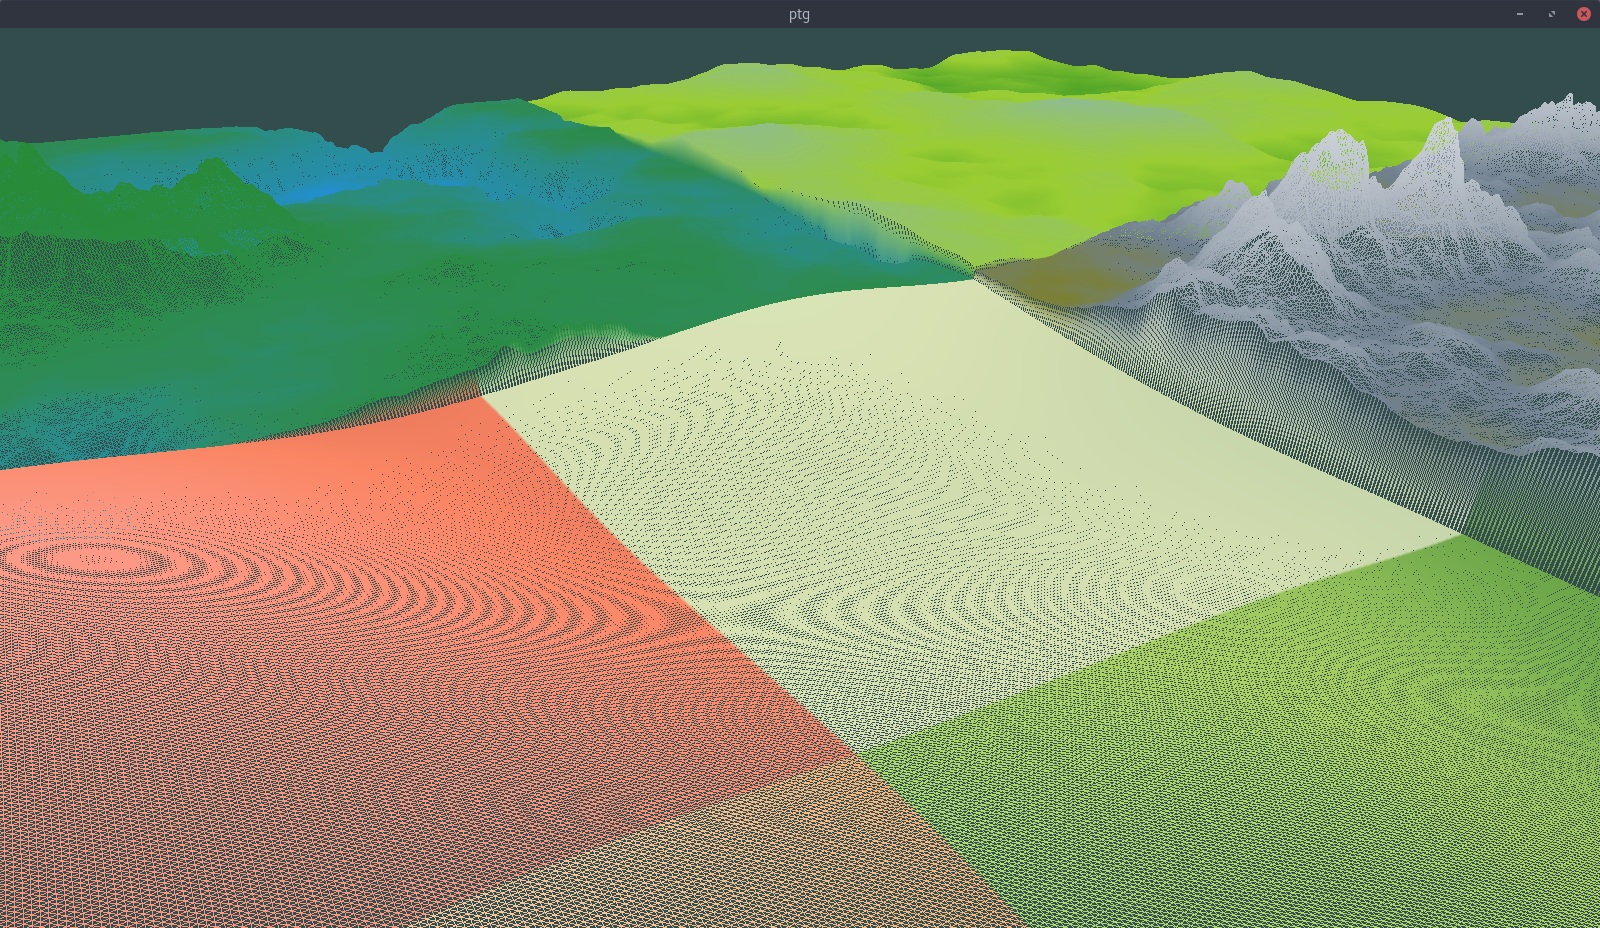
\includegraphics[width=.8\textwidth]
        {img/uffs/interpolationArea/showareanotinterpo.png}
        \caption{Casos de fronteiras}
  \end{figure}
\end{frame}

\begin{frame}{Geração de Terrenos com Biomas Distintos para Jogos}
  \begin{figure}
		\centering
        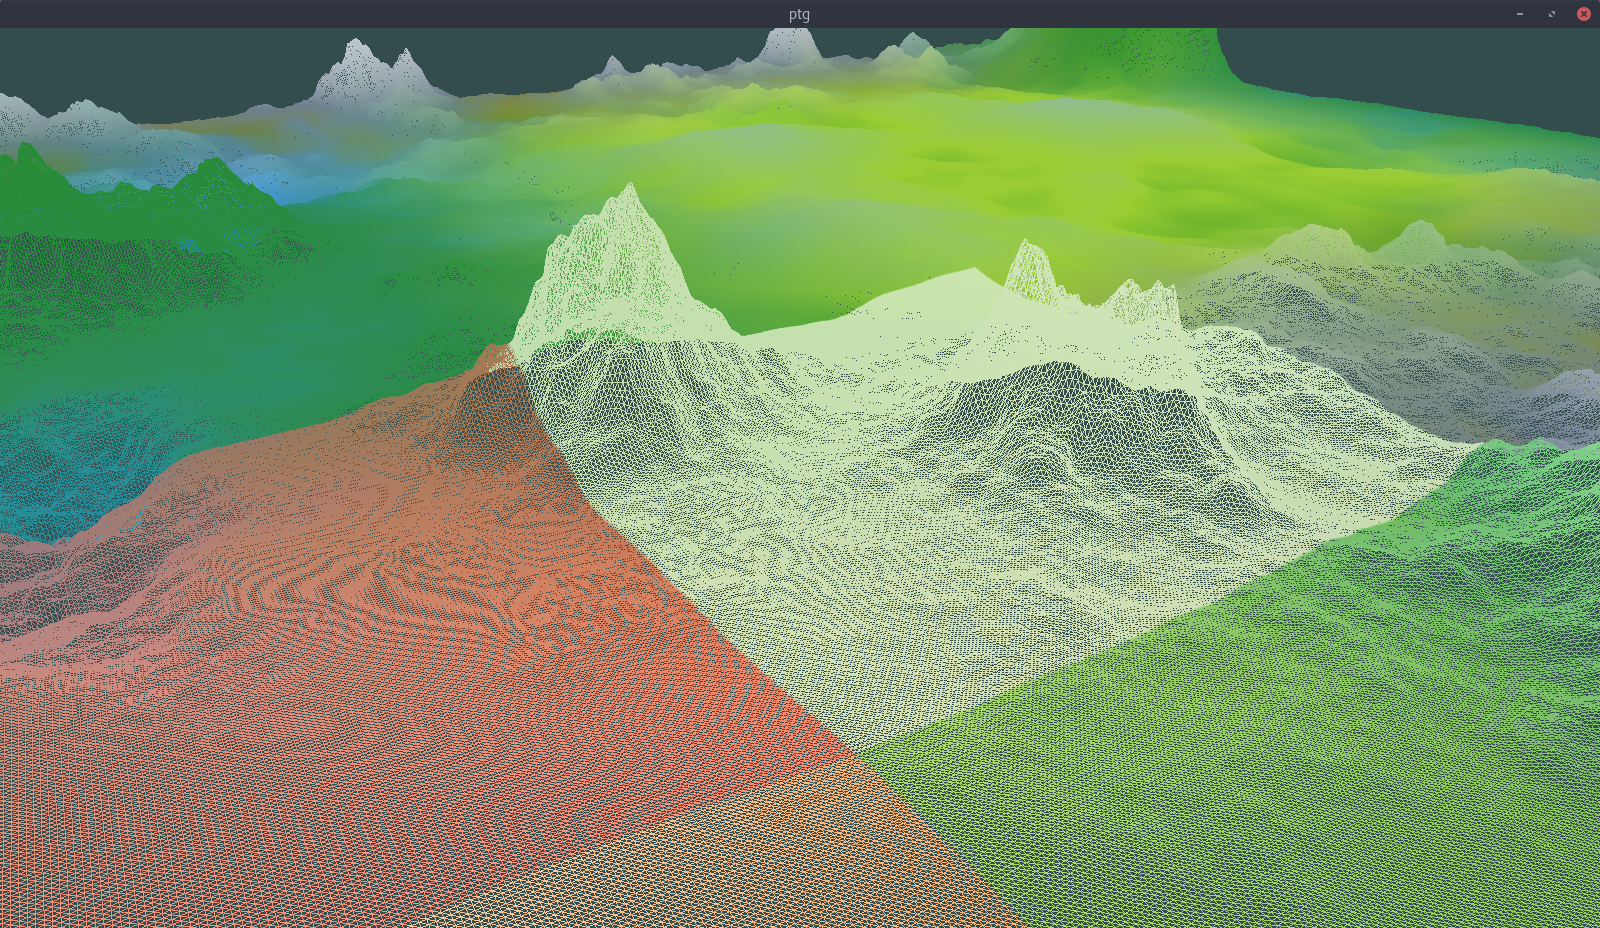
\includegraphics[width=.8\textwidth]
        {img/uffs/interpolationArea/showareainterpolating.png}
        \caption{Com interpolação}
  \end{figure}
\end{frame}

\begin{frame}{Geração de Terrenos com Biomas Distintos para Jogos}
  \begin{figure}
		\centering
        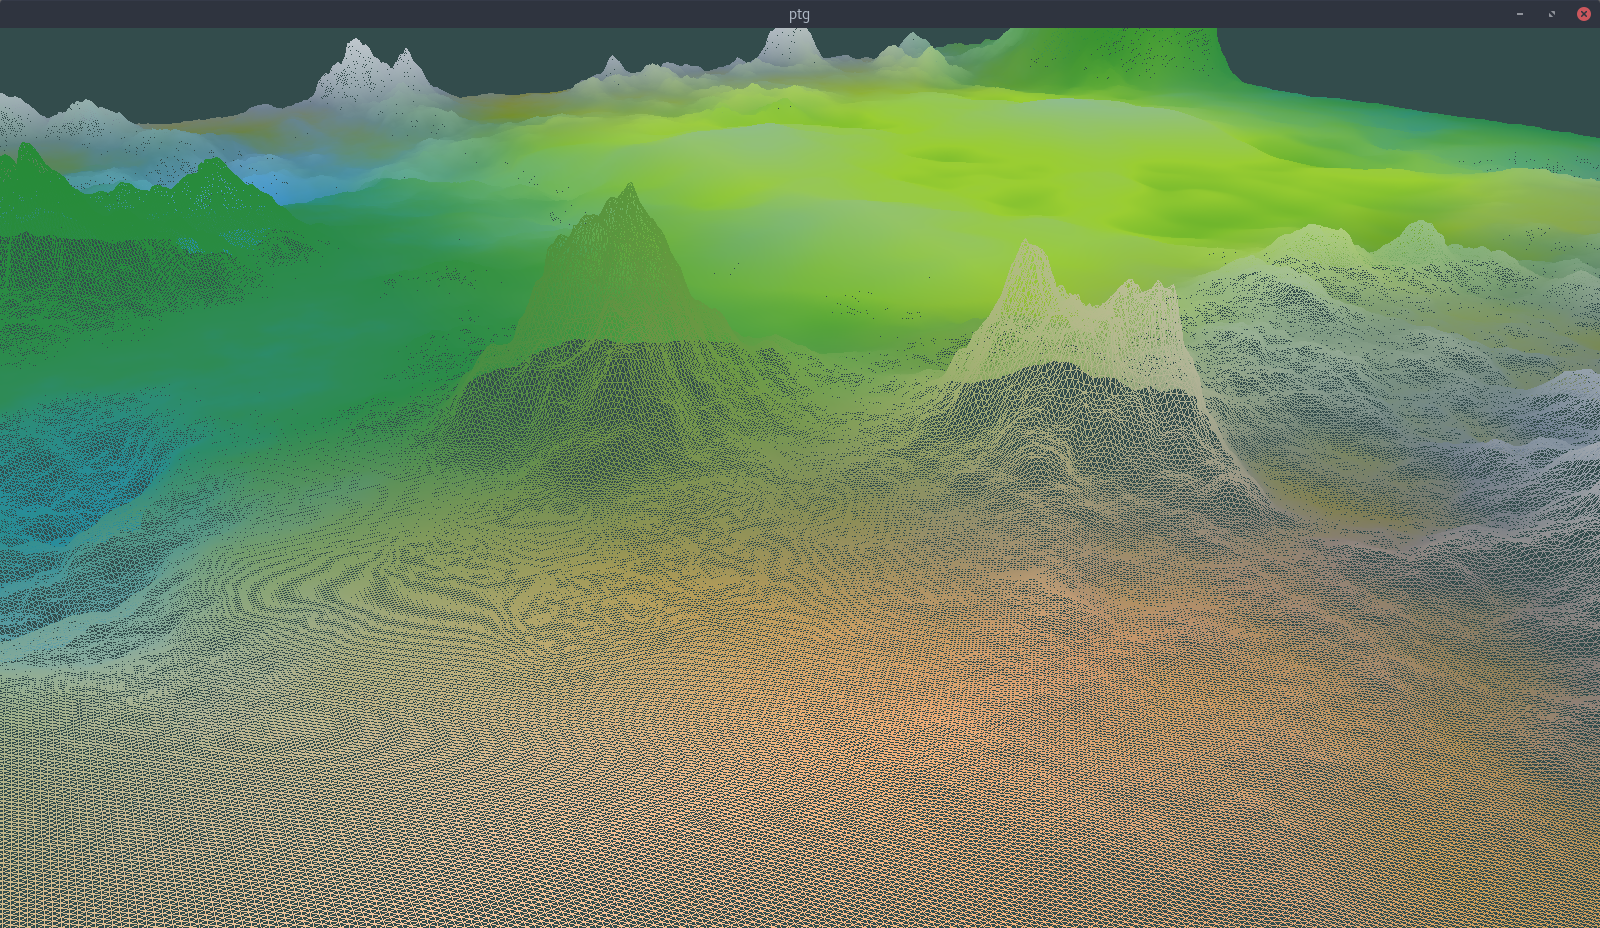
\includegraphics[width=.8\textwidth]{img/uffs/interpolationArea/interpolation.png}
        \caption{Com interpolação}
  \end{figure}
\end{frame}





% Trabalho do Fernando
\begin{frame}{Fernando}
  \begin{itemize}
        \item Trabalho dele \ldots
    \end{itemize}
\end{frame}

\begin{frame}{Fernando}
  \begin{figure}
		\centering
        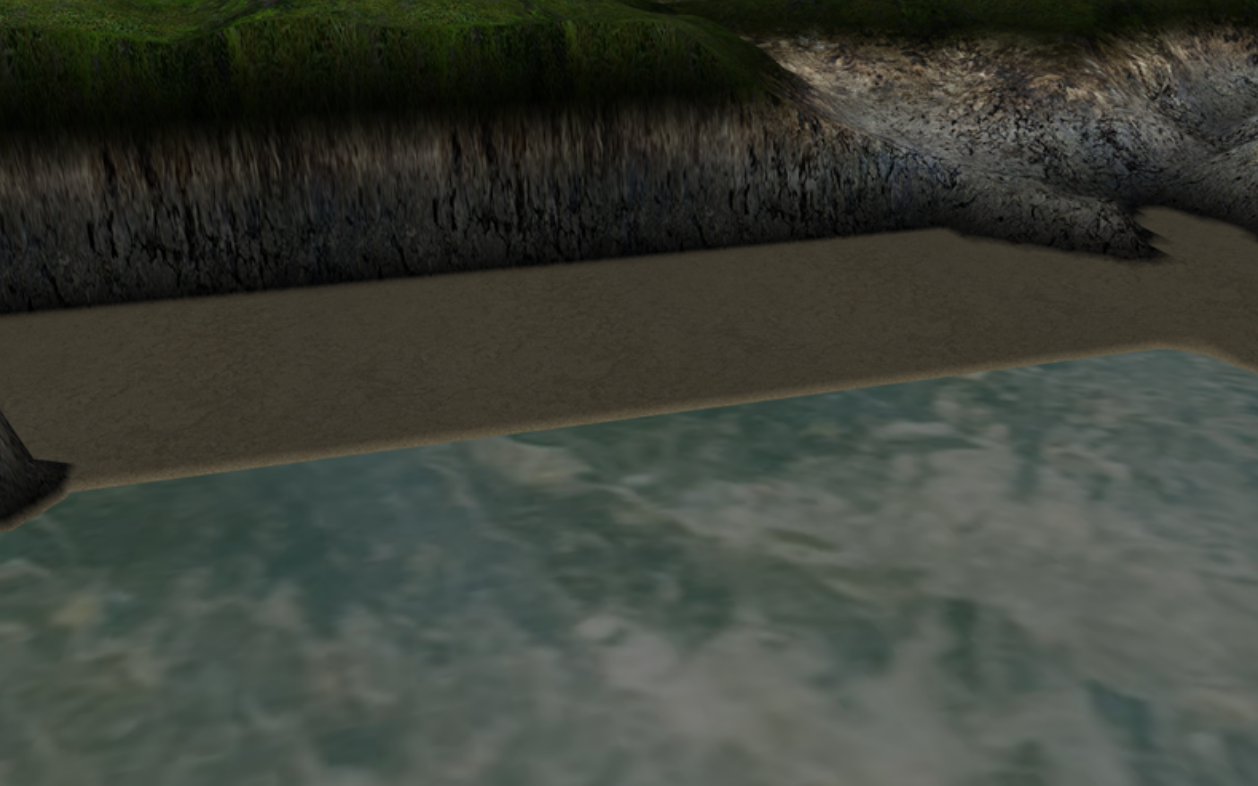
\includegraphics[width=.8\textwidth]
        {img/uffs/fernando/linearcosta.png}
        \caption{Costa linear.}
  \end{figure}
\end{frame}

\begin{frame}{Fernando}
  \begin{figure}
		\centering
        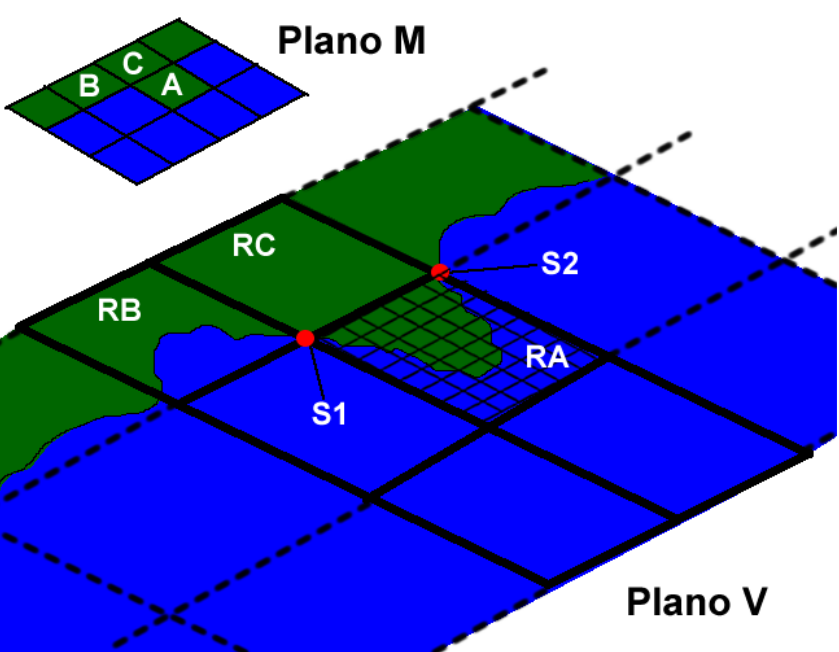
\includegraphics[width=.8\textwidth]{img/uffs/fernando/metodo.png}
        \caption{Método.}
  \end{figure}
\end{frame}

\begin{frame}{Fernando}
  \begin{figure}
		\centering
        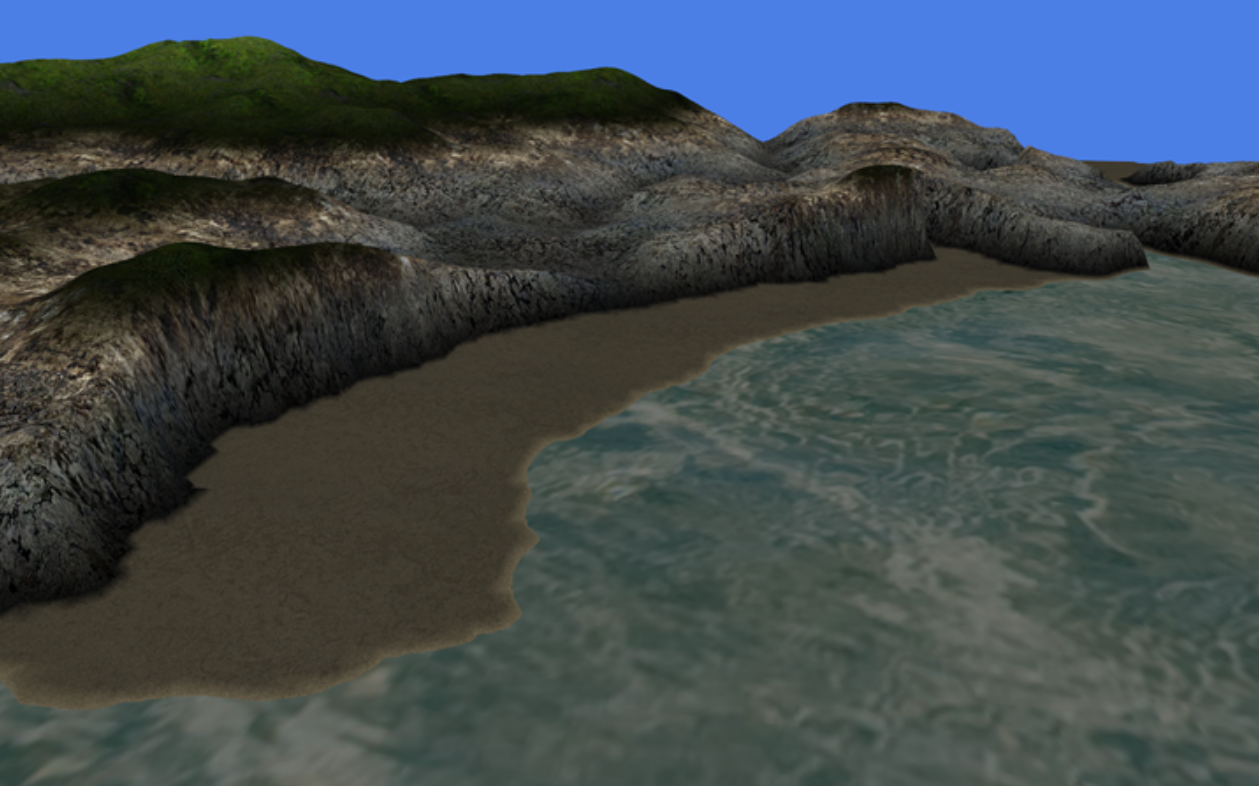
\includegraphics[width=.8\textwidth]
        {img/uffs/fernando/costaorganica.png}
        \caption{Costa orgânica.}
  \end{figure}
\end{frame}